\chapter{Аналитическая часть}
В данном разделе будут рассмотрены теоретические основы задачи коммивояжёра, алгоритма полного перебора и муравьиного алгоритма для решения данной задачи.

\section{Задача коммивояжёра}
Будет рассматриваться графовая формулировка задачи коммивояжёра: необходимо найти кратчайший путь прохода по всем заданным пунктам такой, чтобы каждый пункт был посещён ровно один раз и конечным пунктом оказался тот, с которого был начат обход \cite{item11}. 

В данной работе условия задачи реализуются при помощи взвешенного неориентированного графа, вершины которого представляют города Африки, а веса рёбер~---~расстояния между соответствующими городами. Вес ребра будет больше, если прямой путь между городами лежит через пустыню, и меньше, если пусть проходит через водоём (кроме рек).

На карте Африки были выбраны города, соединённые линией на рисунке \ref{img:map}.

\begin{table}[h!]
  \centering
  \begin{tabular}{p{1\linewidth}}
    \centering
    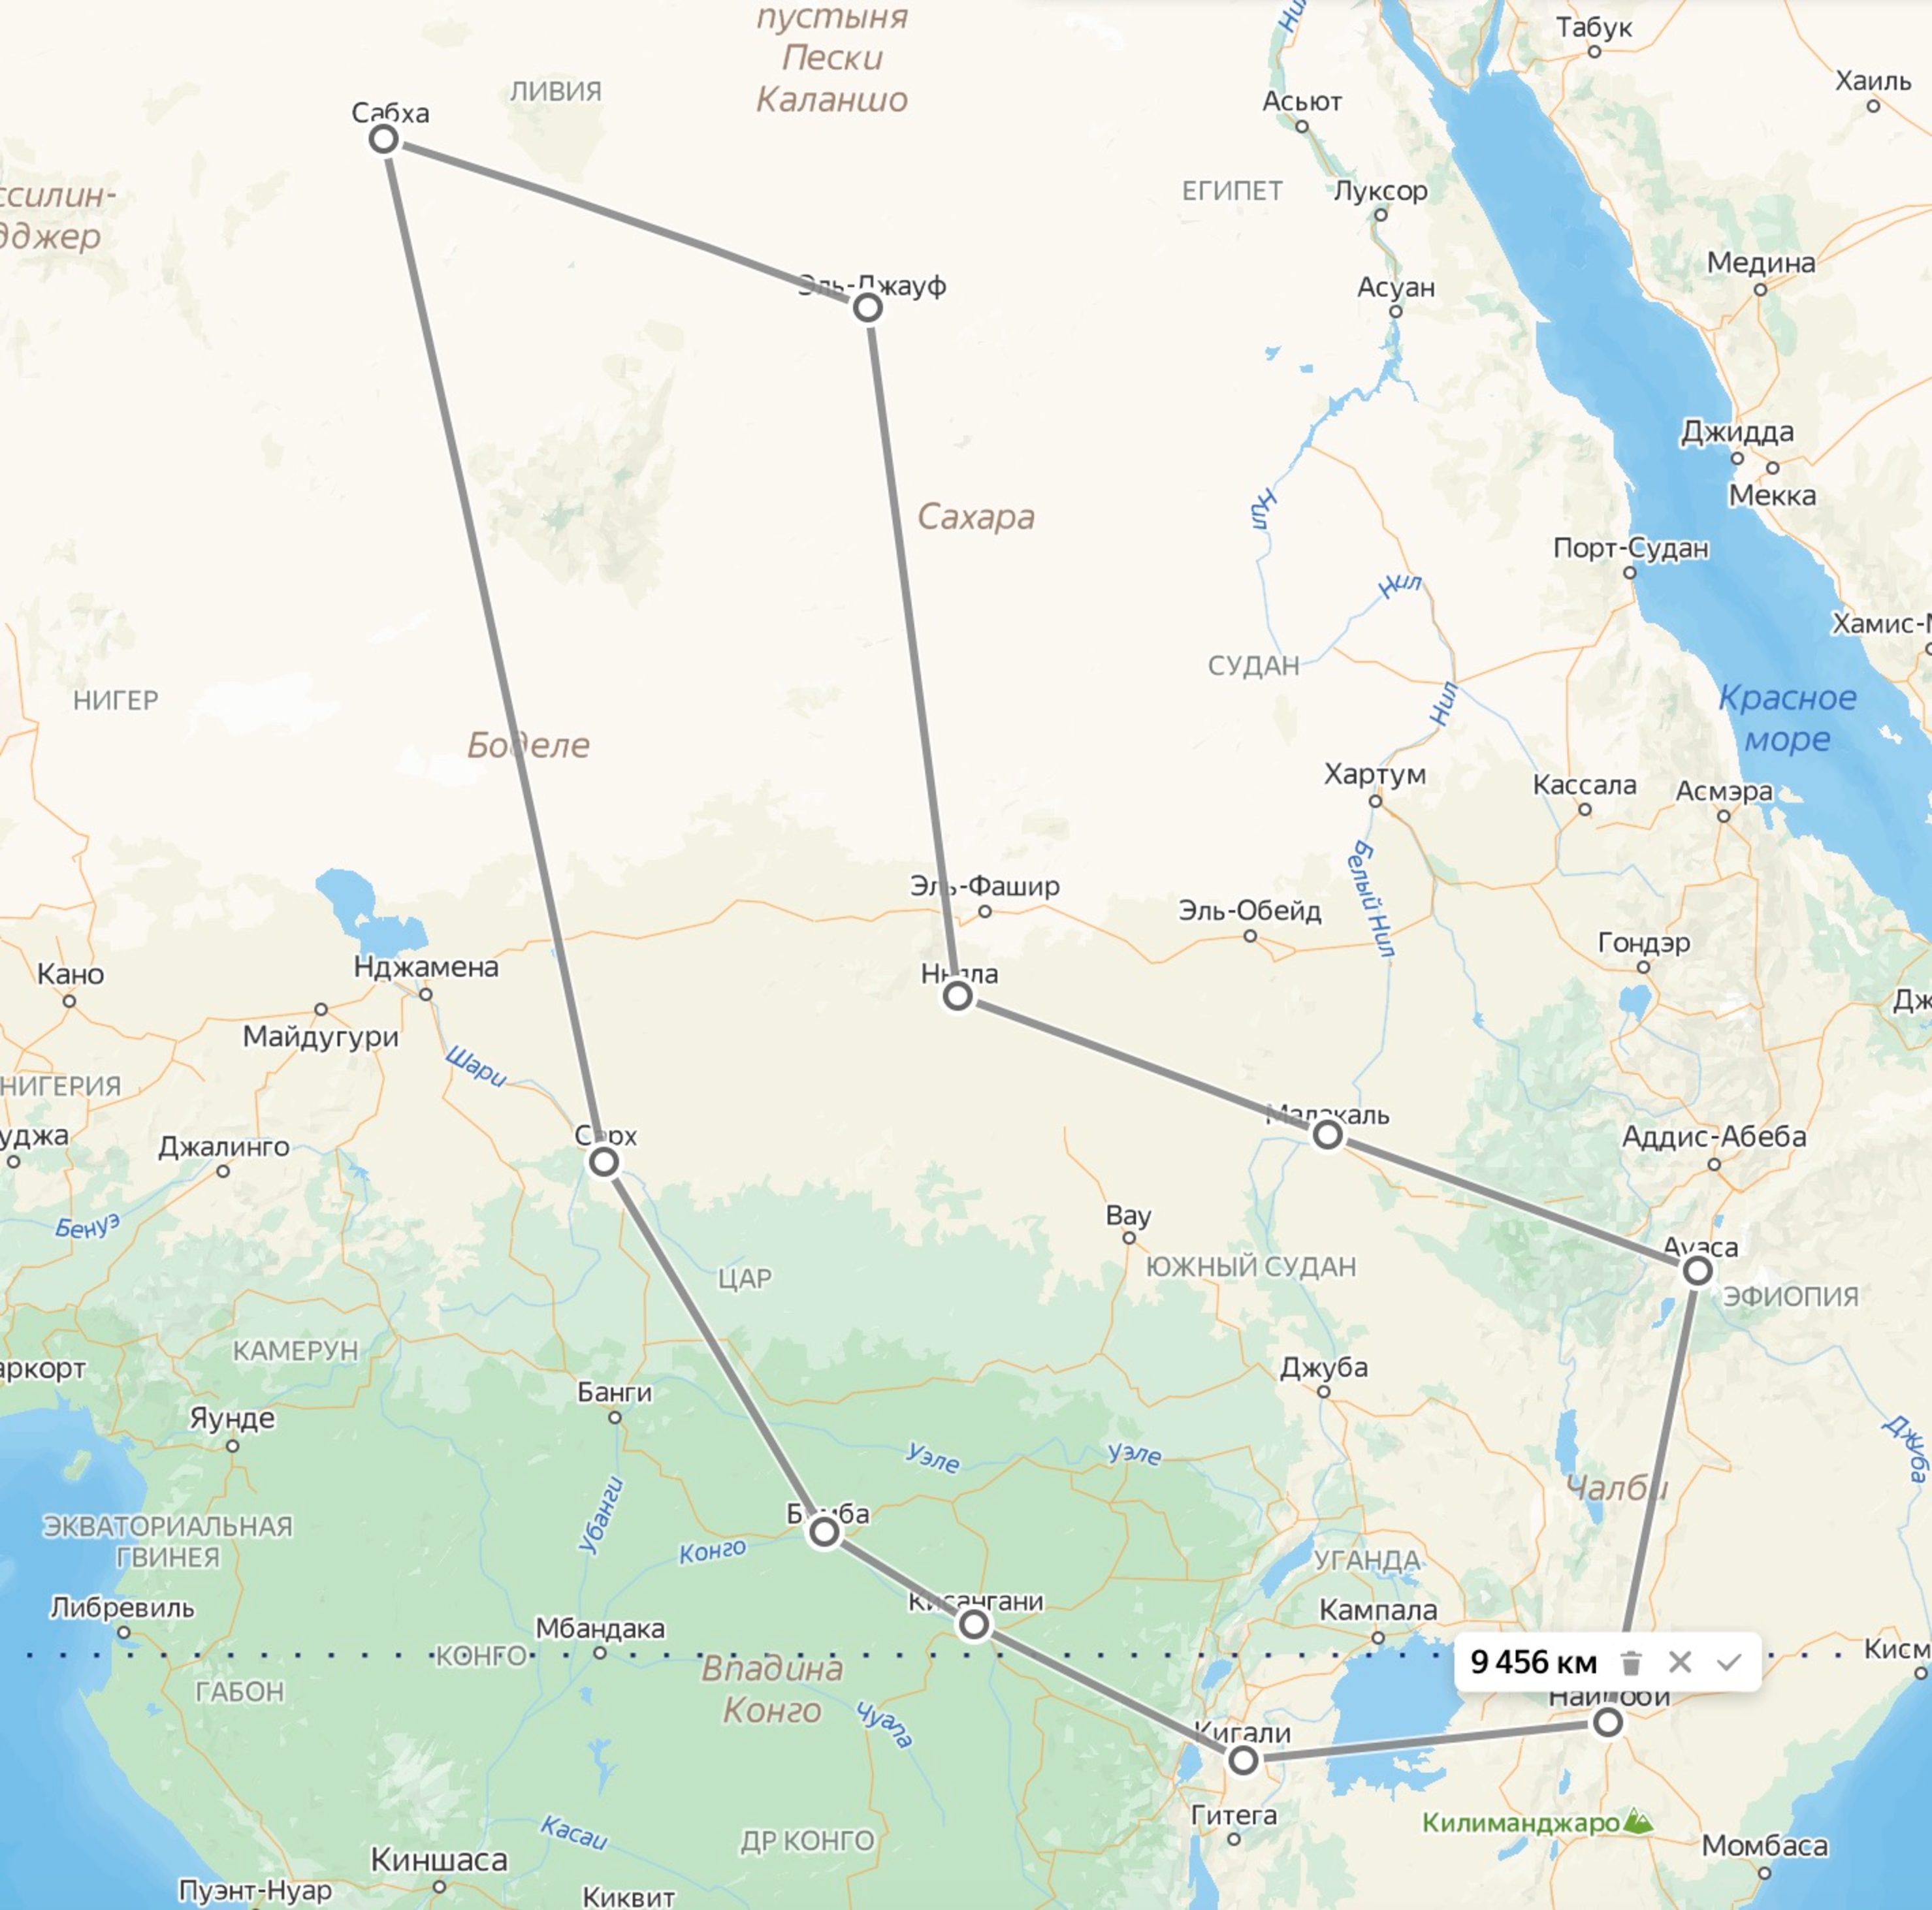
\includegraphics[width=0.55\linewidth]{./images/map.pdf}
    \captionof{figure}{Участок карты Африки с выбранными городами \cite{item13}}
    \label{img:map}
  \end{tabular}
\end{table}

Тогда задача сводится к поиску кратчайшего Гамильтонова цикла, то есть простого элементарного цикла, проходящего через каждую вершину графа \cite{item12}, для неориентированного графа.


\subsection{Алгоритм полного перебора}
Алгоритм полного перебора заключается в переборе всех возможных комбинаций последовательности посещаемых пунктов. Так как число возможных Гамильтоновых циклов на графе конечно, применение этого алгоритма допустимо. 

На вход алгоритму подаётся число городов и матрица смежности графа. Если положить количество городов равным $N$, то в результате работы алгоритма будут рассмотрены все возможные перестановки из $N-1$ элементов. В контексте данной задачи элементами будут номера населённых пунктов~---~вершин графа. Для каждой перестановки рассчитывается суммарная длина перемещений. В результате будет выбрана последовательность посещения населённых пунктов такая, при которой суммарное перемещение будет наименьшим. 

\subsection{Муравьиный алгоритм}
Муравьиный алгоритм основывается на имитации механизмов самоорганизации муравьев, обеспечивающих достижение системой определённой цени благодаря взаимодействию низкоуровневых элементов \cite{item14}. Эти элементы, то есть муравьи, коммуницируют за счёт стигмерджей~---~тип взаимодействия, при котором одна сторона изменяет определённую часть окружающей среды, а остальные используют эту информацию, когда находятся в данной окрестности. Биологически это осуществимо через выделение муравьём феромона~---~стойкого вещества, которое, будучи воспринятым другими муравьями, указывает им, куда стоит двигаться, подчиняя стадному инстинкту. Чем больше феромона в определённой области, тем больше муравьёв ранее было в этой области. Соответственно привлекательность этой области для следующего муравья повышается. 

В ходе решения задачи моделируется решение задачи коммивояжёра муравьиной колонией за $t$ суток. Пусть задан граф из $N$ городов и дана его матрица смежности $D$. Полагается, что колония обладает некоторой глобальной памятью~---~информация о распределении феромона по рёбрам графа должна где-то храниться, например, в виде матрицы. Матрица феромона заполняется некоторым небольшим значением по умолчанию. В начале каждых суток каждый муравей колонии, размер которой устанавливается равным количеству вершин графа, то есть $N$, размещается в одном из городов. Начальные позиции муравьёв не совпадают. За день каждый муравей проходит полный Гамильтонов цикл по графу, действуя независимо от других особей.

Для муравья устанавливаются следующие компетенции:
\begin{itemize}
	\item Зрение~---~означает, что муравей может оценить ребро по его длине: более длинное ребро будет менее привлекательным для муравья. В связи с этим, желание муравья посетить $j$-ый город описывается соотношением \begin{equation}
		\eta_{ij} = \frac{1}{D_{ij}}, \quad \text{где $D_{ij}$~---~длина ребра между пунктами $i$ и $j$.}
	\end{equation}
	\item Память~---~означает, что муравей помнит, какие пункты посещал ранее. Уже посещённые пункты вычёркиваются из списка непосещённых пунктов, в который изначально заносятся номера всех вершин графа, кроме начальной позиции данного муравья. Далее список непосещённых вершин для $k$-ого муравья будет обозначаться $J_k$.
	\item Обоняние~---~означает, что муравей способен чувствовать концентрацию феромона $\tau_{ij}$ на ребре между пунктами $i$ и $j$. Тогда чем выше концентрация феромона на ребре, тем больше желание муравья пойти по данному ребру.
\end{itemize}

Учитывая перечисленные компетенции можно вывести формулу для расчёта вероятности посещения $k$-ым муравьём, находящимся в вершине $i$, вершины  $j$:
\begin{equation} \label{eqn:1}
	P_{ij,k}(t) = \begin{cases}
		0, \quad \text{если $j \in J_k$,} \\
		\frac{\left[\eta_{ij}\right]^{\beta} \cdot \left[\tau_{ij}\right]^{\alpha}}{\sum_{q \notin J_k} \left[\eta_{iq}\right]^{\beta} \cdot \left[\tau_{iq}\right]^{\alpha}}, \quad \text{иначе.}
	\end{cases}
\end{equation}

В формуле (\ref{eqn:1}) $\alpha$~---~это коэффициент стадности, задающий вес концентрации феромона при вычислении вероятности, а $\beta$~---~коэффициент жадности, определяющий вес длины ребра, причём $\alpha,\beta \in (0,1)$. В случае, когда $\alpha = 0$, алгоритм вырождается в жадный, то есть всегда будет выбираться ближайший к текущей позиции город. В случае, когда $\beta = 0$, алгоритм становится стадным, что влечёт за собой преждевременный приход к одному субоптимальному решению.

Если муравей сумел пройти маршрут, удовлетворяющий понятию Гамильтонова цикла, на пройденных им рёбрах должна возрасти концентрация феромона в соответствии со следующей формулой:
\begin{equation} \label{eqn:3}
	\tau_{ij}(t + 1) = (1 - \rho) \cdot \tau_{ij}(t) + \sum_{k=1}^m \Delta\tau_{ij,k}(t),
\end{equation}
где $\rho \in (0,1)$~---~коэффициент испарения феромона с течением времени, $m$~---~количество муравьёв в колонии, $\tau_{ij}(t + 1)$~---~концентрация феромона на ребре между пунктами $i$ и $j$ в наступающий день, $\tau_{ij}(t)$~---~концентрация феромона на ребре между пунктами $i$ и $j$ в уходящий день, $\tau_{ij,k}(t)$~---~концентрация феромона на ребре между пунктами $i$ и $j$ в наступающий день для $k$-ого муравья, а $\Delta\tau_{ij,k}(t)$ определяется по формуле \begin{equation}\label{eqn:2}
	\Delta\tau_{ij,k}(t) = \begin{cases}
		\frac{Q}{L_k(t)}, \quad (i,j) \in T_k(t), \\
		0, \quad (i,j) \notin T_k(t).
	\end{cases}
\end{equation}

В формуле (\ref{eqn:2}) $Q$~---~параметр, имеющий значение порядка длины оптимального пути, $L_k(t)$~---~длина маршрута $k$-ого муравья, $T_k(t)$~---~маршрут, пройденный $k$-ым муравьём к моменту времени $t$. 

Значение $Q$ может быть рассчитано единожды в начале работы алгоритма по формуле \begin{equation}
	Q = \frac{\sum_{i=1}^n \sum_{j=1}^n D_{ij}}{N}.
\end{equation}

Формулой (\ref{eqn:3}) учитывается естественное испарение феромона за ночь и его прирост за счёт проходов муравьиной колонии за предыдущий день. В случае, если значение феромона на ребре стало слишком мало, нужно вновь восстановить его до значения по умолчанию, иначе некоторые непосещённые пункты станут недостижимыми.

Для улучшения временных характеристик вводят элитных муравьев, которые дополнительно усиливают рёбра наилучшего маршрута, найденного с начала работы алгоритма. Для $e$ элитных муравьёв рёбра наилучшего маршрута получат следующее усиление концентрации феромона: \begin{equation}
	\Delta\tau_{e} = e \cdot \frac{Q}{L^+}, \quad \text{где $L^+$~---~длина наилучшего маршрута.}
\end{equation}

В результате работы алгоритма находится кратчайший маршрут среди найденных муравьями. Полученный в результате работы алгоритма маршрут не обязательно совпадёт с решением, которое можно получить с помощью алгоритма полного перебора, ввиду неточности муравьиного алгоритма \cite{item14}. Он гарантирует лишь получение близкого к идеальному значения.



















\newpage